\pdfminorversion=4
\documentclass[aspectratio=169]{beamer}

\mode<presentation>
{
  \usetheme{default}
  \usecolortheme{default}
  \usefonttheme{default}
  \setbeamertemplate{navigation symbols}{}
  \setbeamertemplate{caption}[numbered]
  \setbeamertemplate{footline}[frame number]  % or "page number"
  \setbeamercolor{frametitle}{fg=white}
  \setbeamercolor{footline}{fg=black}
} 

\usepackage[english]{babel}
\usepackage{inputenc}
\usepackage{tikz}
\usepackage{courier}
\usepackage{array}
\usepackage{bold-extra}
\usepackage{minted}
\usepackage[thicklines]{cancel}
\usepackage{fancyvrb}

\xdefinecolor{dianablue}{rgb}{0.18,0.24,0.31}
\xdefinecolor{darkblue}{rgb}{0.1,0.1,0.7}
\xdefinecolor{darkgreen}{rgb}{0,0.5,0}
\xdefinecolor{darkgrey}{rgb}{0.35,0.35,0.35}
\xdefinecolor{darkorange}{rgb}{0.8,0.5,0}
\xdefinecolor{darkred}{rgb}{0.7,0,0}
\definecolor{darkgreen}{rgb}{0,0.6,0}
\definecolor{mauve}{rgb}{0.58,0,0.82}

\title[2023-03-06-awkwardforth-for-atlas]{All about AwkwardForth}
\author{Jim Pivarski}
\institute{Princeton University -- IRIS-HEP}
\date{March 6, 2023}

\usetikzlibrary{shapes.callouts}

\begin{document}

\logo{\pgfputat{\pgfxy(0.11, 7.4)}{\pgfbox[right,base]{\tikz{\filldraw[fill=dianablue, draw=none] (0 cm, 0 cm) rectangle (50 cm, 1 cm);}\mbox{\hspace{-8 cm}
\includegraphics[height=1 cm]{princeton-logo-long.png}\hspace{0.1 cm}\raisebox{0.1 cm}{
\includegraphics[height=0.8 cm]{iris-hep-logo-long.png}}\hspace{0.1 cm}}}}}

\begin{frame}
  \titlepage
\end{frame}

\logo{\pgfputat{\pgfxy(0.11, 7.4)}{\pgfbox[right,base]{\tikz{\filldraw[fill=dianablue, draw=none] (0 cm, 0 cm) rectangle (50 cm, 1 cm);}\mbox{\hspace{-8 cm}
\includegraphics[height=1 cm]{princeton-logo.png}\hspace{0.1 cm}\raisebox{0.1 cm}{
\includegraphics[height=0.8 cm]{iris-hep-logo.png}}\hspace{0.1 cm}}}}}

% Uncomment these lines for an automatically generated outline.
%\begin{frame}{Outline}
%  \tableofcontents
%\end{frame}

% START START START START START START START START START START START START START

\begin{frame}{Introduction: what is AwkwardForth?}
\begin{center}
\begin{minipage}{0.89\linewidth}
\large\setlength{\baselineskip}{0.55 cm}

\vspace{0.5 cm}
AwkwardForth is an internal DSL within Awkward Array for accelerating sequential (non-columnar) data-ingest processes that must be discovered at runtime, avoiding a JIT-compilation toolchain as a dependency because Awkward Array is a foundational library.

\vspace{0.5 cm}
\uncover<2->{It has a stable API because an external package, Uproot, uses it heavily.}

\vspace{0.5 cm}
\uncover<3->{Because of all the qualifications in its justification, I doubt other projects would ever need it.}
\end{minipage}
\end{center}
\end{frame}

\begin{frame}{Conclusions}
\large
\begin{itemize}
\item You probably don't need it.
\end{itemize}
\end{frame}

\begin{frame}{\mbox{ }}
\Huge
\begin{center}
\textcolor{darkblue}{\bf BACKUP}
\end{center}
\end{frame}

\begin{frame}{Uproot-Awkward problem (for more-complex-than-jagged-arrays)}
\vspace{0.25 cm}
\only<1>{
\includegraphics[width=\linewidth]{PLOTS/awkward-uproot-interaction-1.pdf}}\only<2>{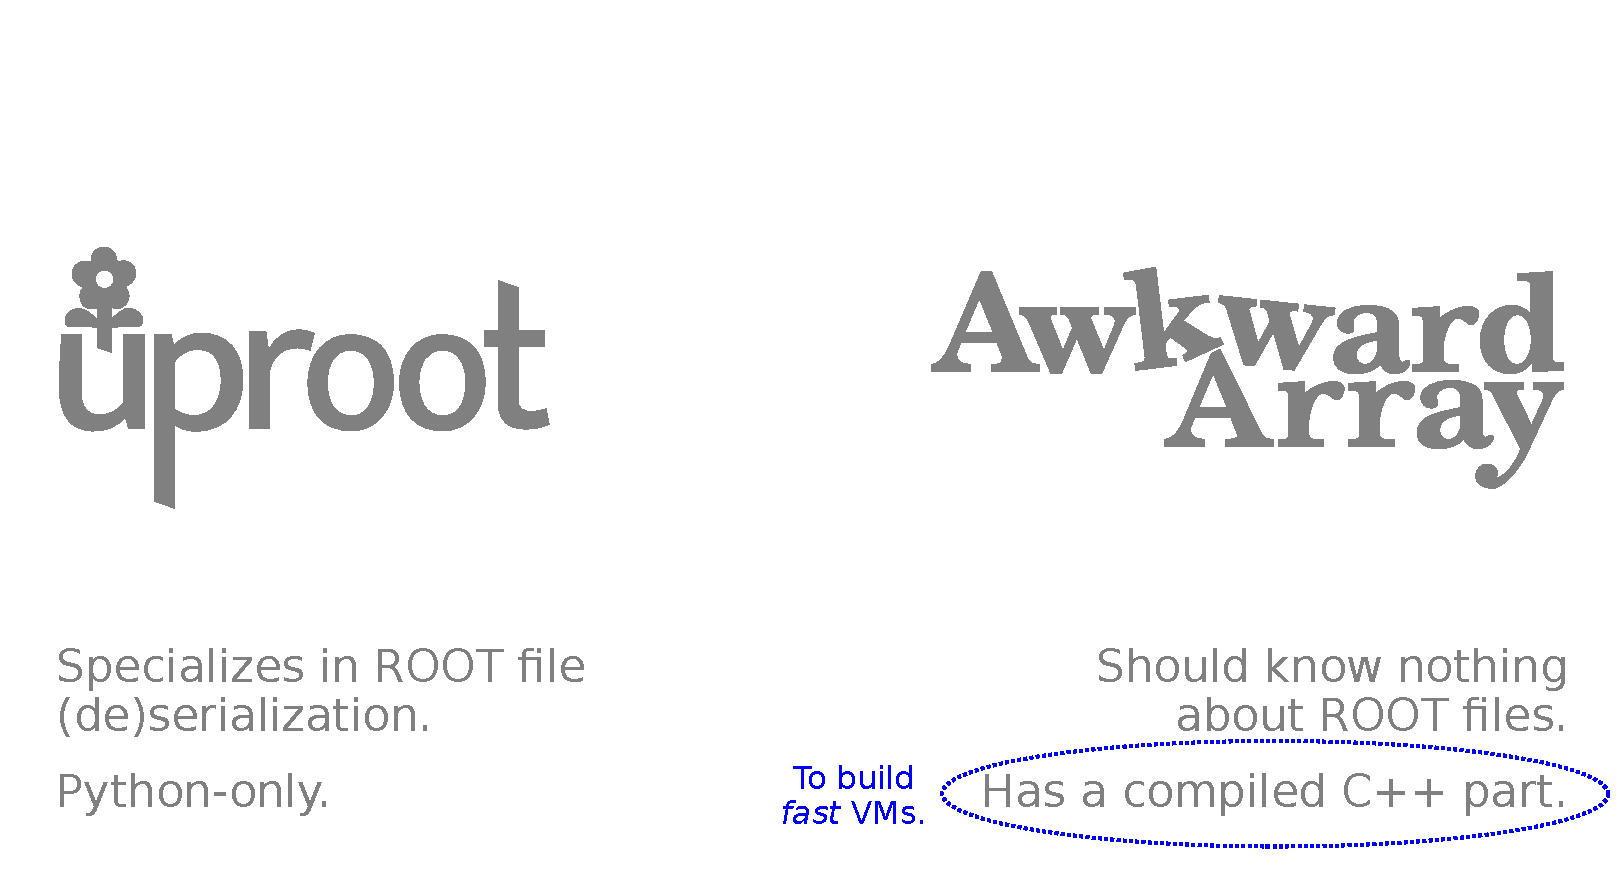
\includegraphics[width=\linewidth]{PLOTS/awkward-uproot-interaction-2.pdf}}\only<3>{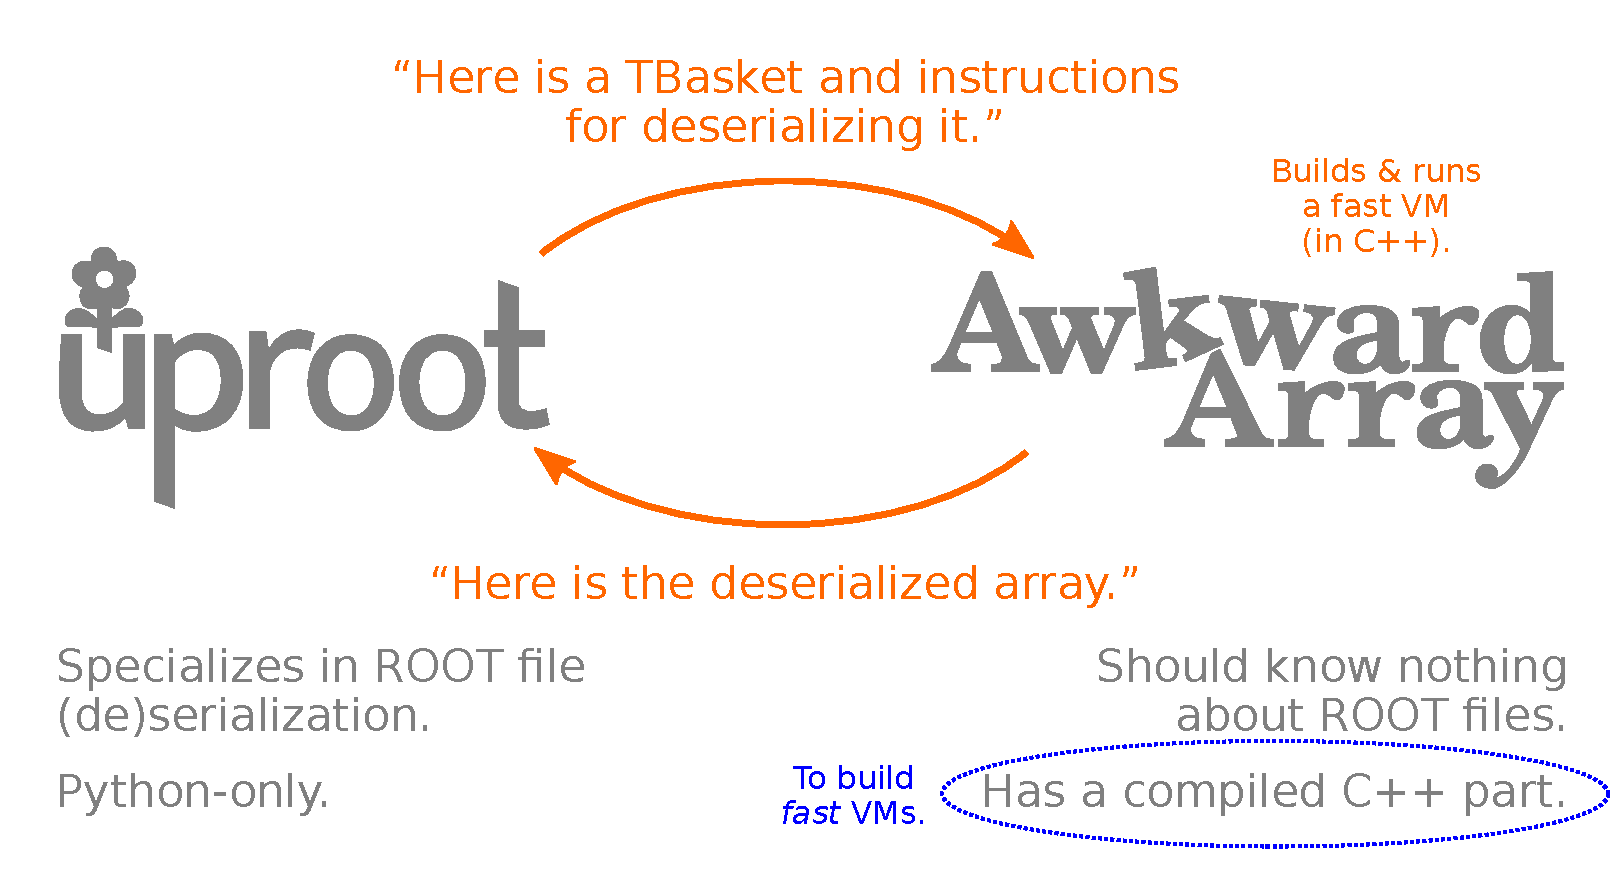
\includegraphics[width=\linewidth]{PLOTS/awkward-uproot-interaction-3.pdf}}
\end{frame}

\begin{frame}{We need a deserialization language; why Forth?}
\vspace{0.5 cm}
Forth was promoted in the early 1980's as an alternative to complex languages. It was the only language capable of running fast (compile-like speeds) within memory constraints of the first Macintosh.

\vspace{0.5 cm}
\begin{columns}
\column{0.5\linewidth}
\centering
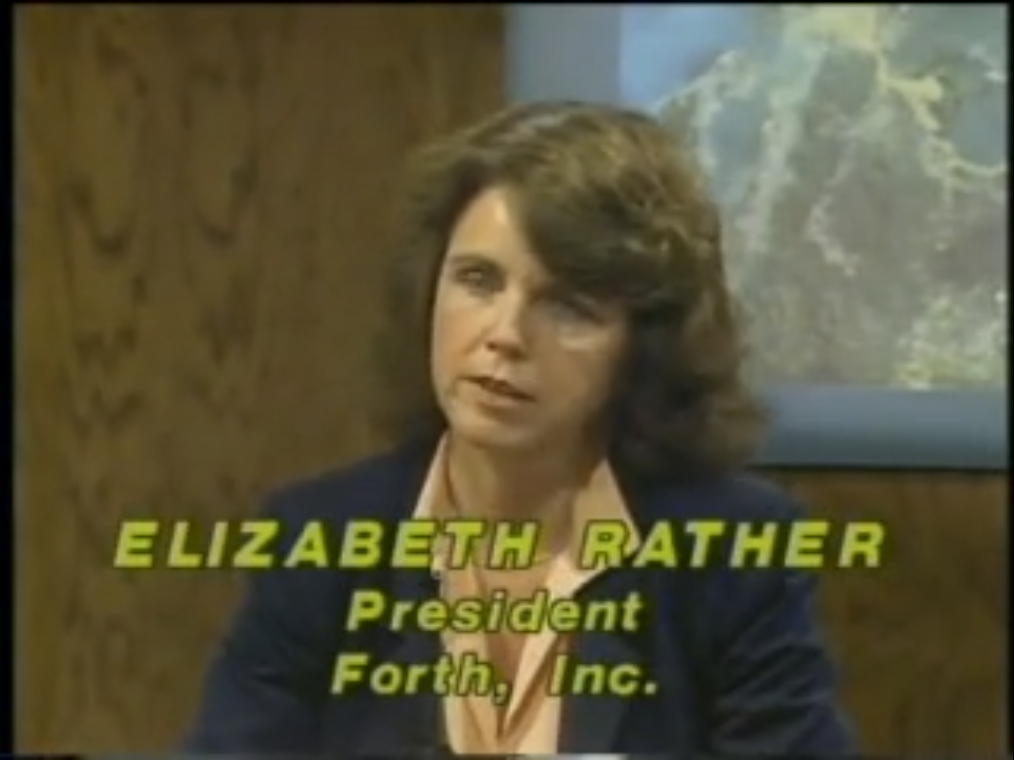
\includegraphics[height=5 cm]{PLOTS/elizabeth-rather-the-computer-chronicles.png}

\column{0.5\linewidth}
\centering
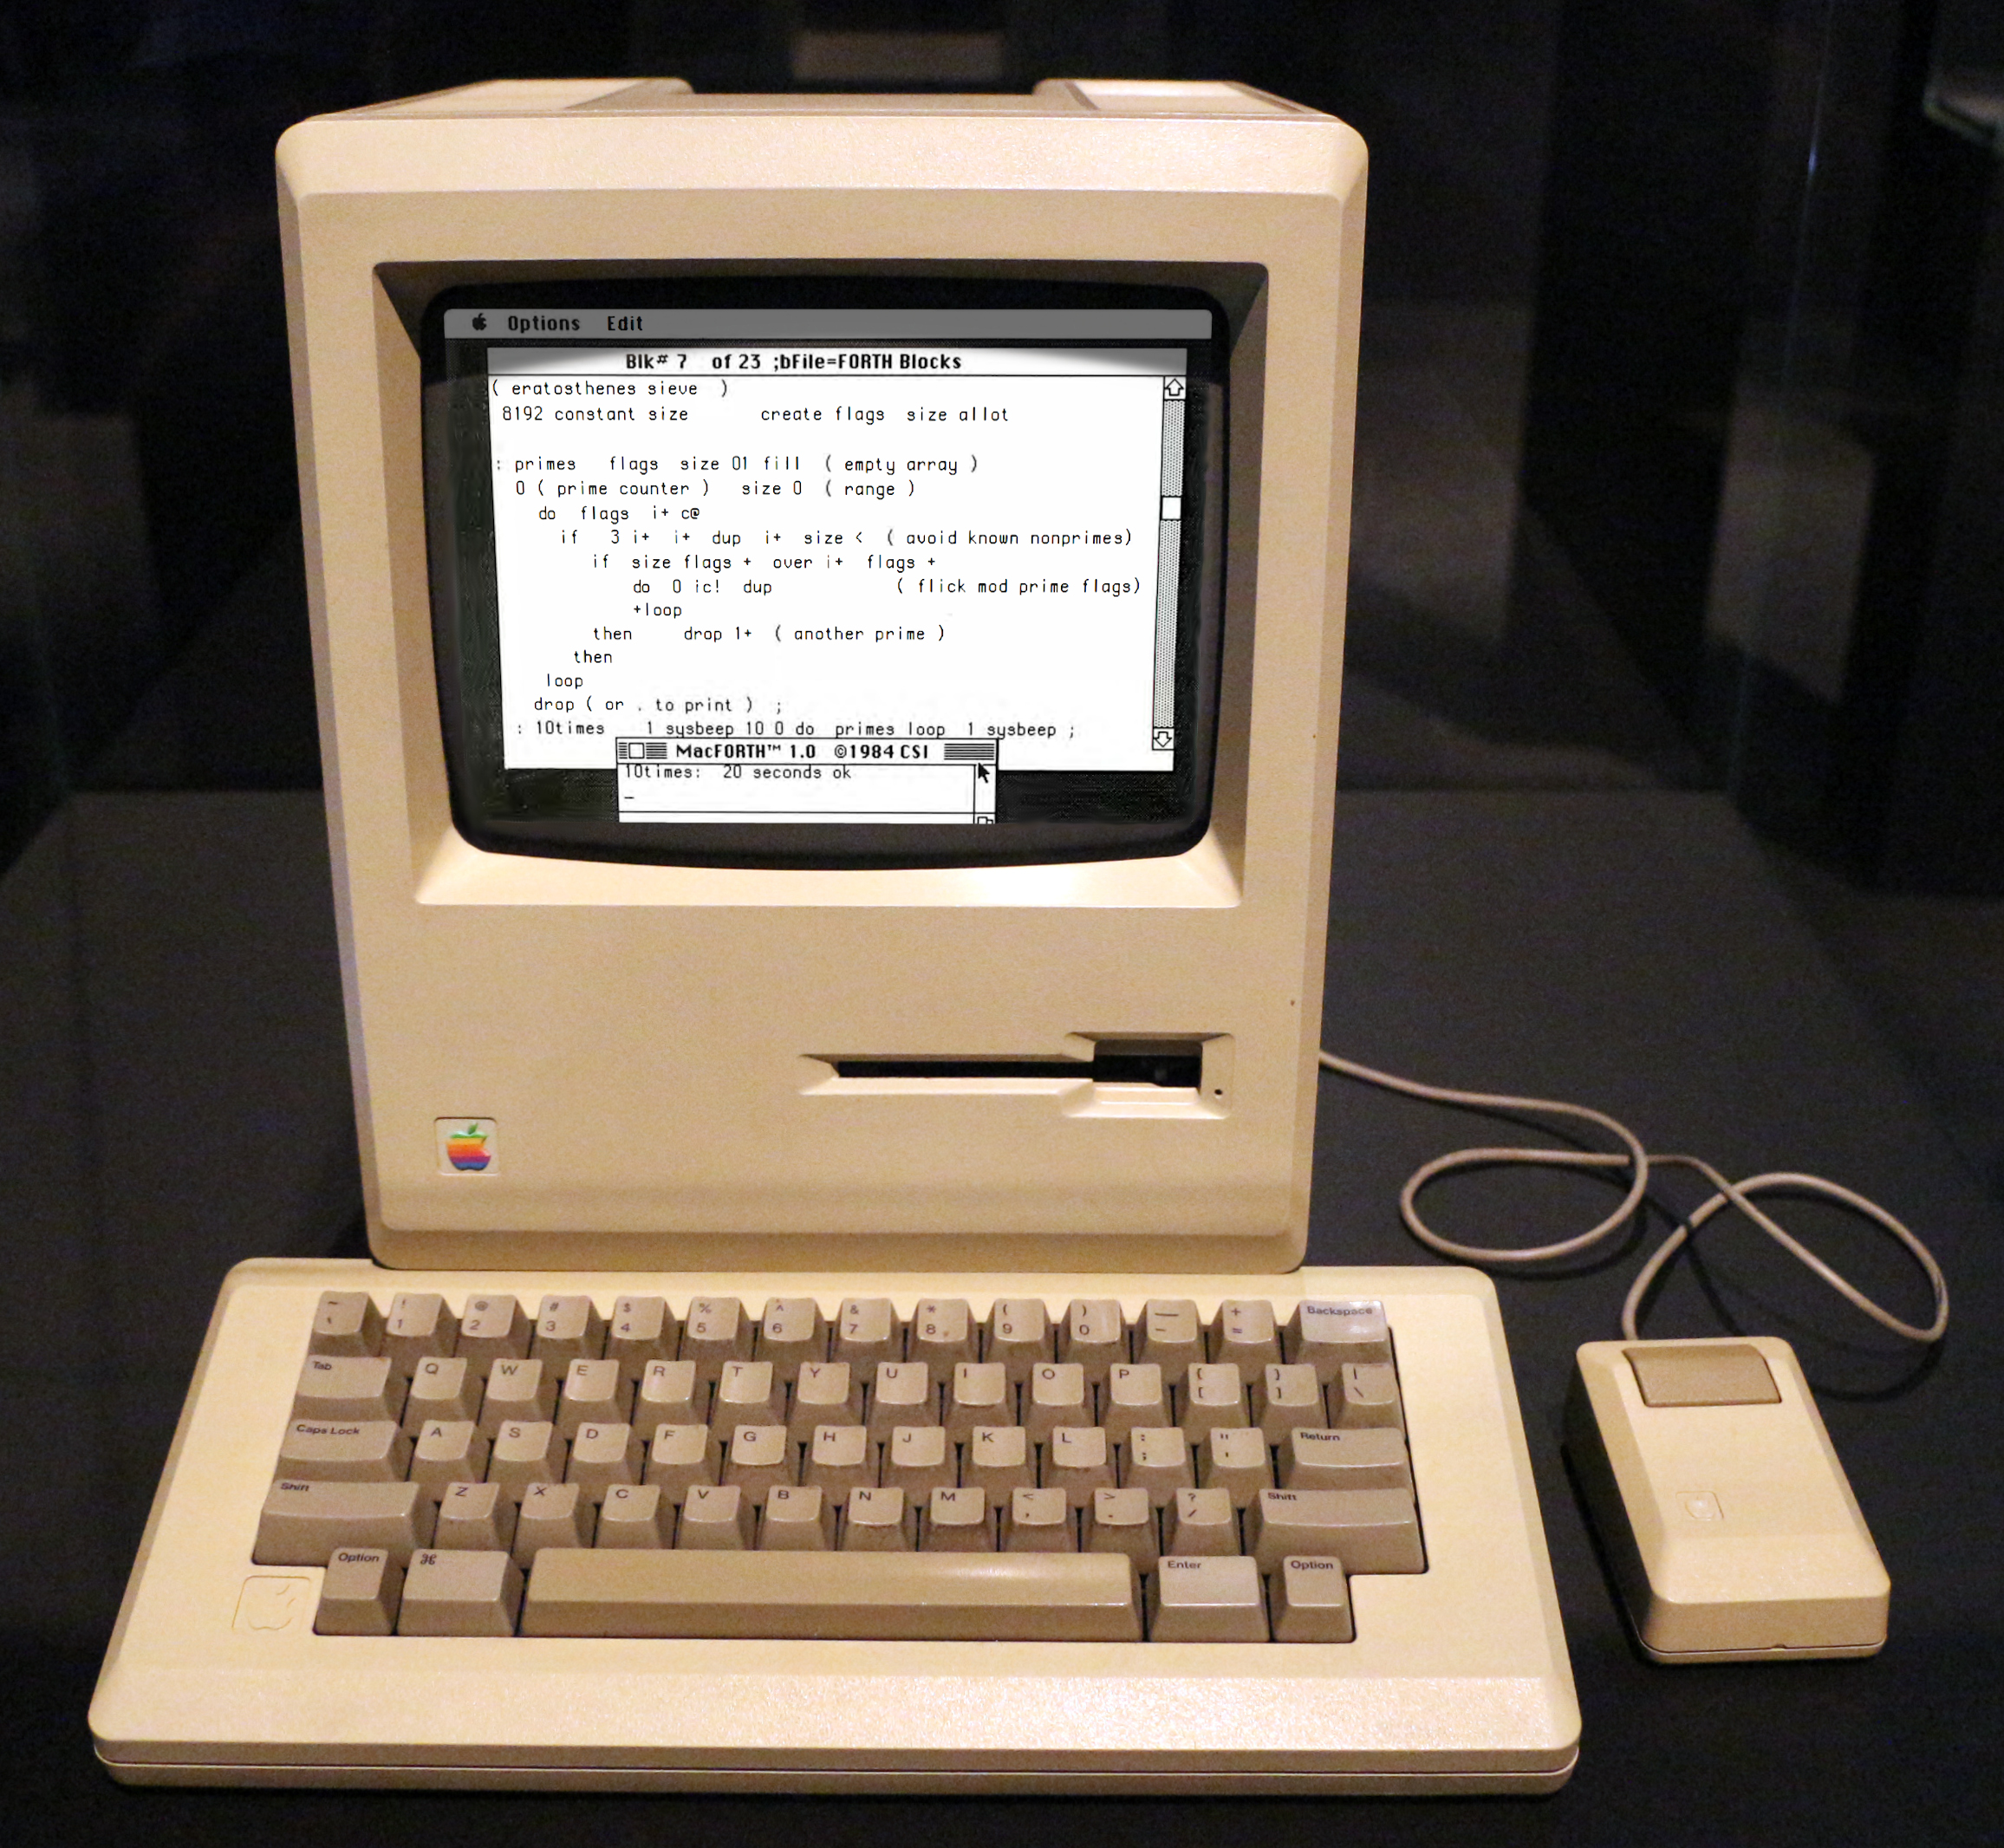
\includegraphics[height=5 cm]{PLOTS/macintosh-forth-code.jpg}
\end{columns}
\end{frame}

\begin{frame}{What Forth looks like (good for code generation!)}
\vspace{0.25 cm}
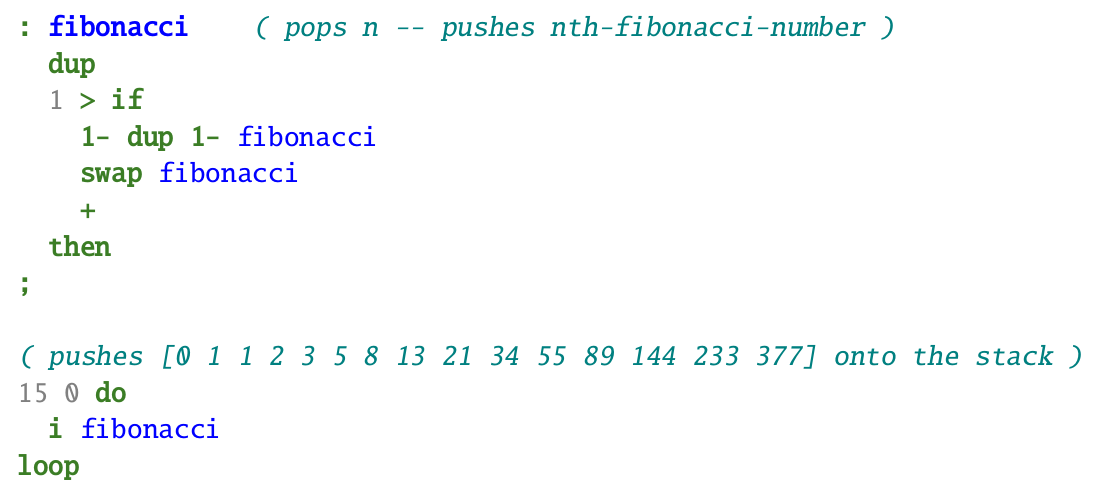
\includegraphics[width=0.9\linewidth]{PLOTS/forth-example.png}

\vspace{0.5 cm}
Almost no syntax; each whitespace-separated word performs an action on a stack of integers. This stack is the only data. Apart from the lack of jumps and the ability to define new words, it's essentially an assembler for a virtual stack-based machine.
\end{frame}

\begin{frame}{Adapted for data-ingest}
\vspace{0.25 cm}
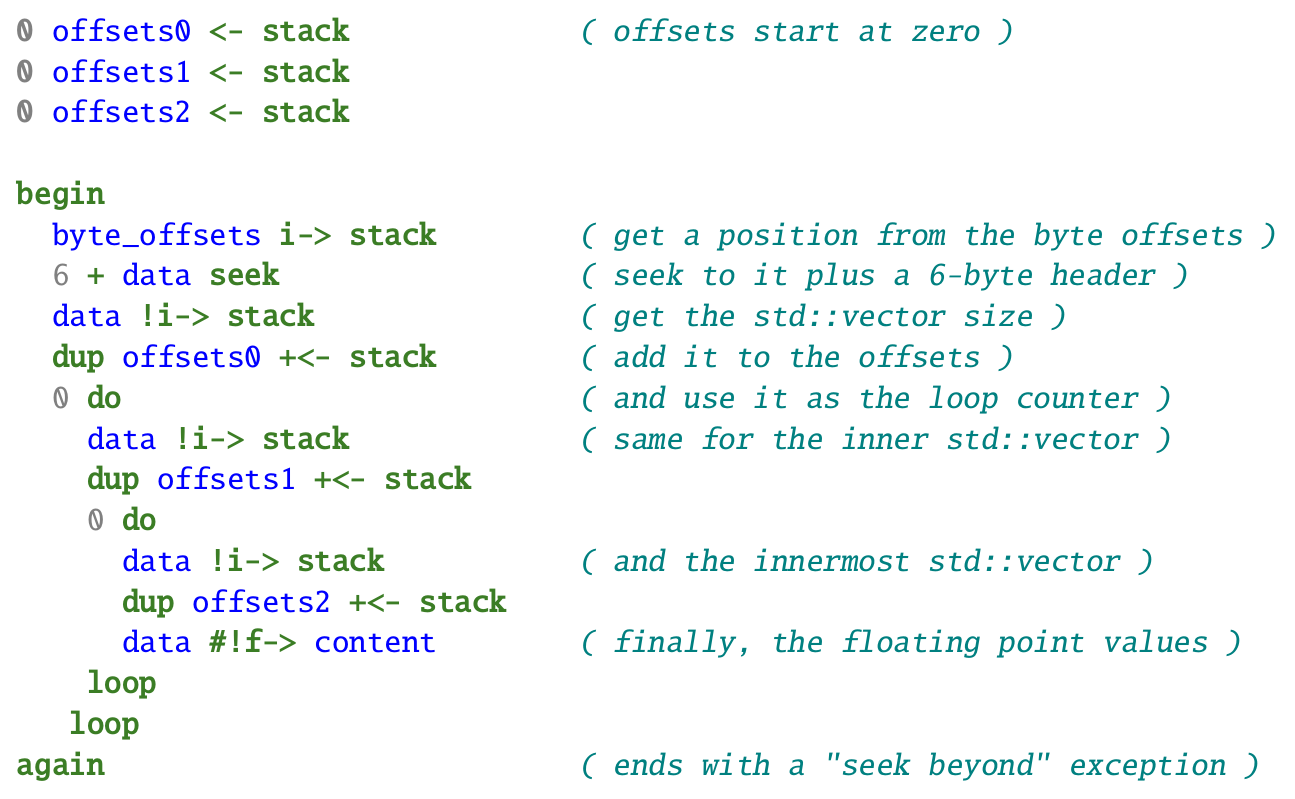
\includegraphics[width=0.9\linewidth]{PLOTS/forth-parsing-example.png}
\end{frame}

\begin{frame}{The language was implemented two years ago}
\vspace{0.17 cm}
\begin{columns}
\column{1.15\linewidth}
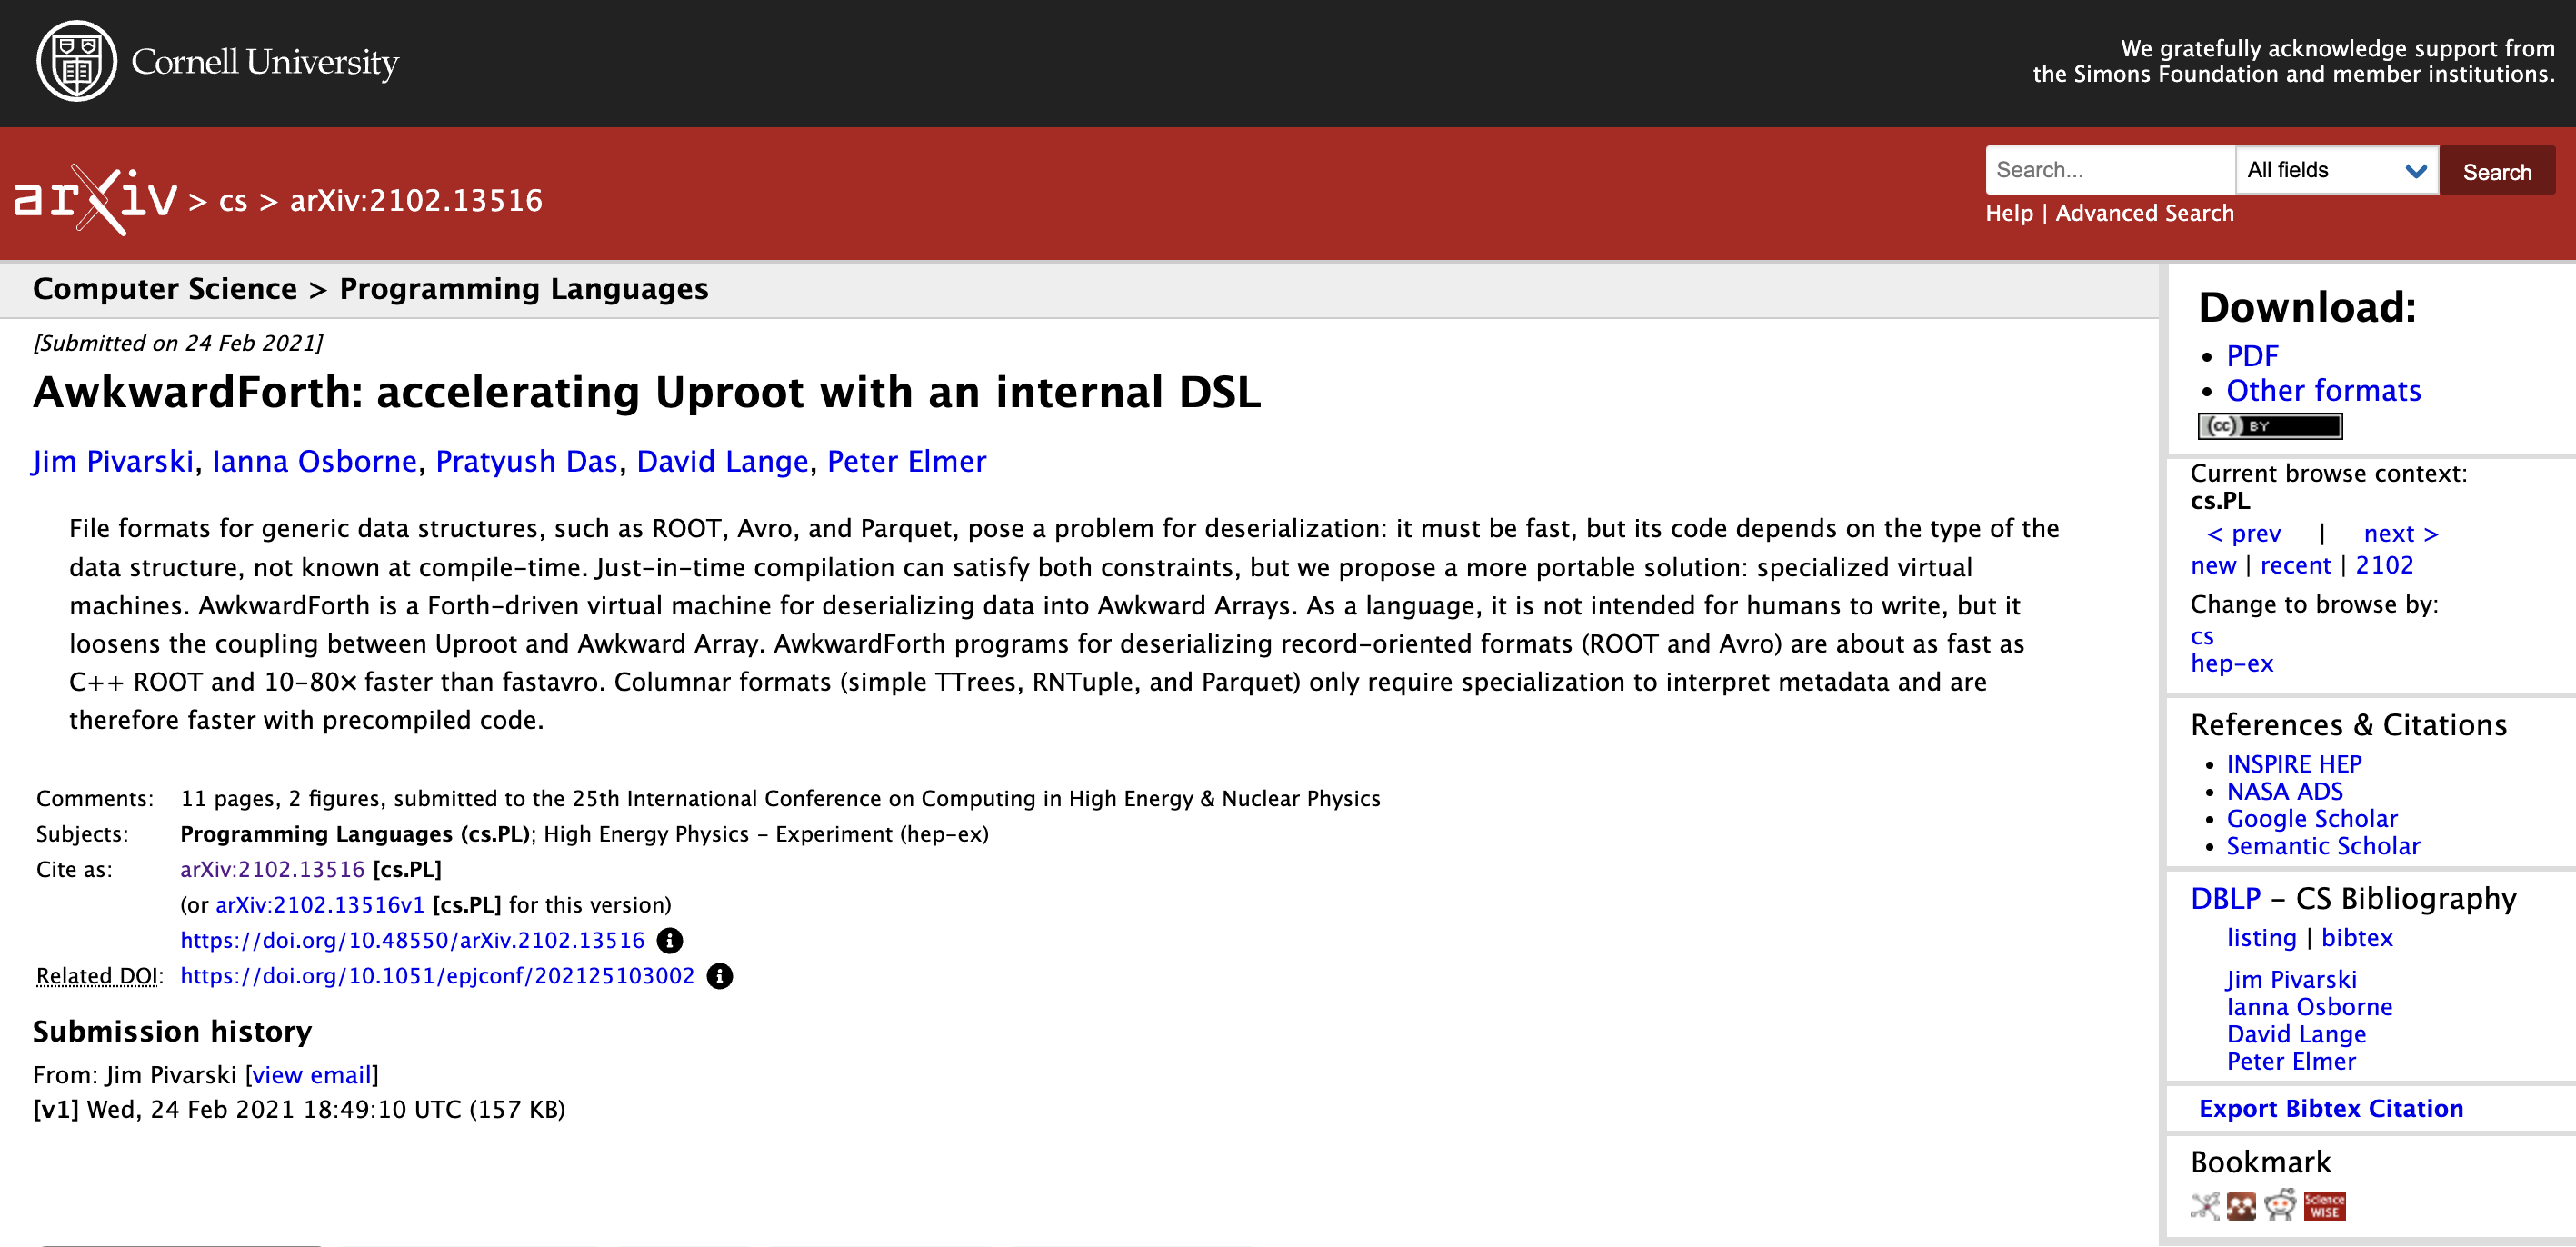
\includegraphics[width=\linewidth]{PLOTS/AwkwardForth-paper.png}
\end{columns}
\end{frame}

\begin{frame}{Uproot was updated to use it last summer (version 5.0)}
\vspace{0.17 cm}
\begin{columns}
\column{1.15\linewidth}
new paper here
\end{columns}
\end{frame}

\begin{frame}{The language is fully documented}
\vspace{0.17 cm}
\begin{columns}
\column{1.15\linewidth}
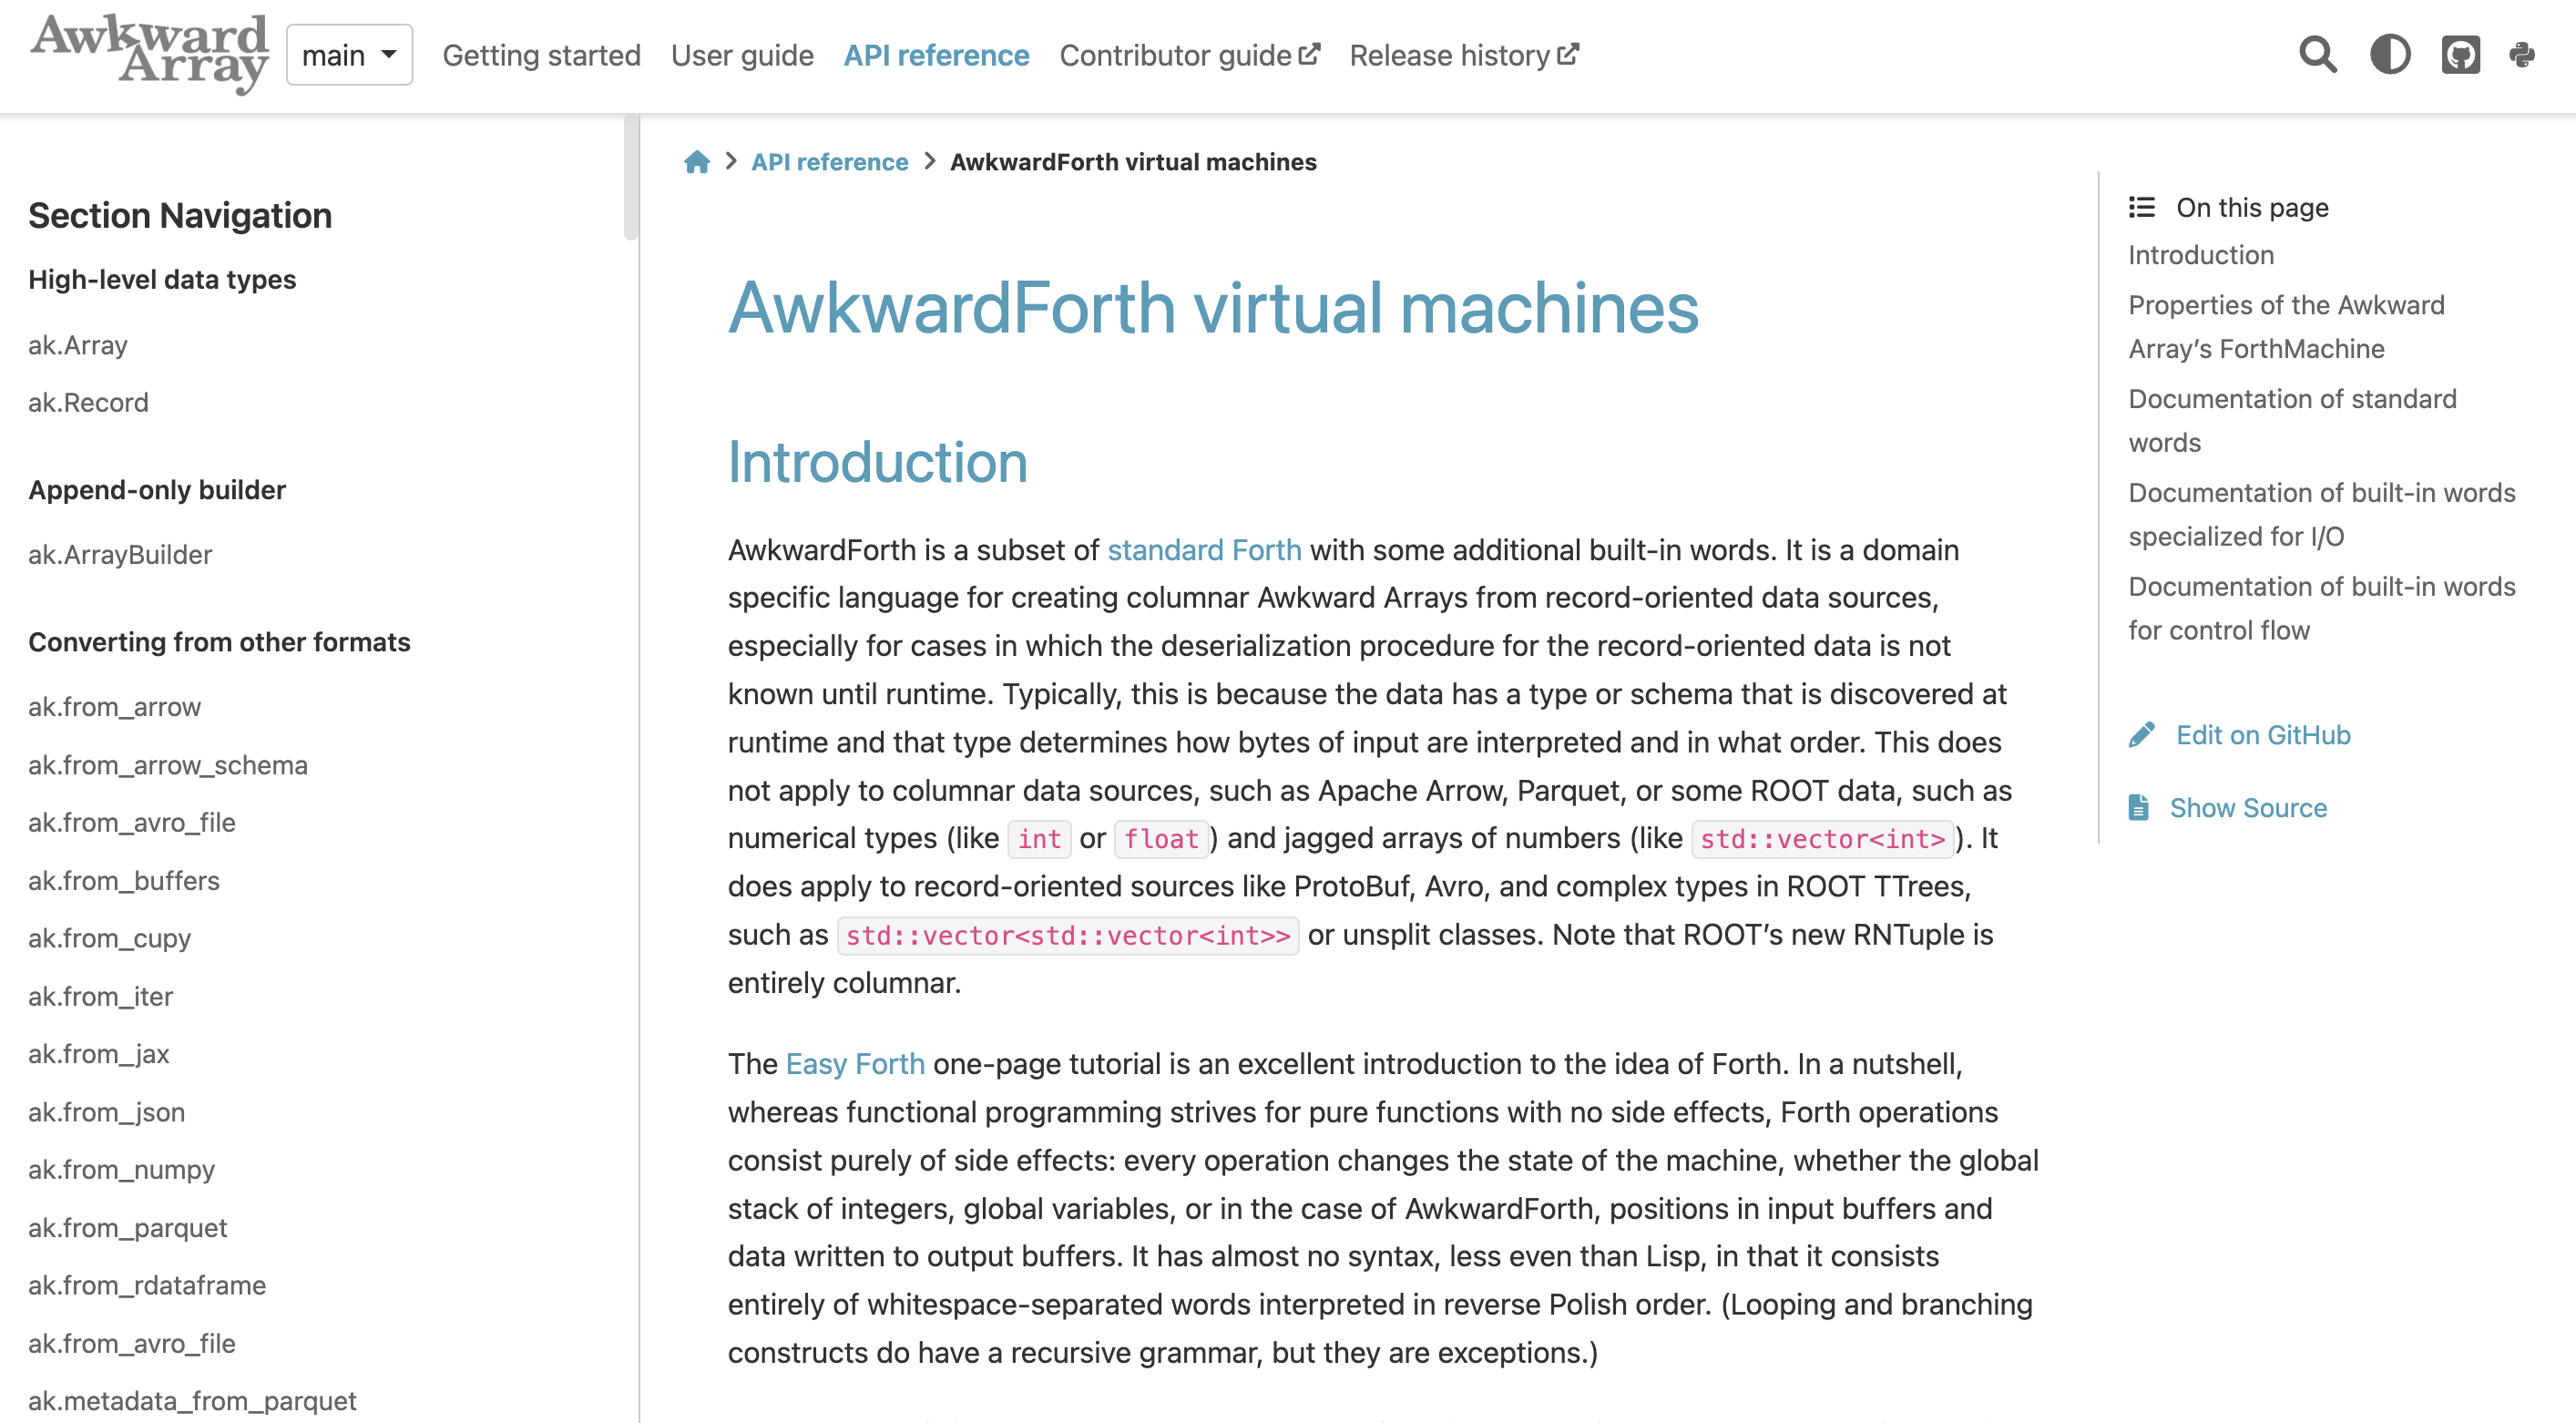
\includegraphics[width=\linewidth]{PLOTS/AwkwardForth-documentation.png}
\end{columns}
\end{frame}






\end{document}
